\subsection{Coil:Cooling:DX}\label{coilcoolingdx}

This coil input structure is meant to supplant the coil objects from previous EnergyPlus versions (Coil:Cooling:DX:SingleSpeed, Coil:Cooling:DX:TwoSpeed, Coil:Cooling:DX:MultiSpeed, etc.). This coil input structure uses a combination of four objects to fully define the performance of the coil under a range of operating conditions.

\begin{enumerate}
\def\labelenumi{\arabic{enumi}.}
\item Coil:Cooling:DX - Defines where the coil's evaporator and condenser sections are connected to the HVAC system through node connections to air loops or zones (if condenser section rejects heat to a zone), as well as the coil's availability.

\item Coil:Cooling:DX:CurveFit:Performance - Defines how the coil operates over a range of operating conditions.

\item Coil:Cooling:DX:CurveFit:OperatingMode - Defines the rated coil characteristics (capacity, evaporator section air flow rate, etc.) and capacity control method for a given operating mode. Operating modes are generally used to describe humidity control strategies for DX cooling coil arrangements that enable enhanced dehumidification.

\item Coil:Cooling:DX:CurveFit:Speed - Defines DX cooling coil performance for a specific speed within a single operating mode.
\end{enumerate}
Note: The Coil:Cooling:DX:CurveFit:Performance object also allows users to input 3 operating modes: Base Operating Mode, Alternative Operating Mode 1, and Alternative Operating Mode 2. When the Base Operating Mode is an only mode input, the coil performs like a regular cooling DX coil and no specific dehumidification capability. The alternative operating mode 1 is used for enhanced dehumidification. When all 3 modes are inputs, the coil performs as a subcool reheat coil. When load sensible heat ratio (SHR), defined as sensible cooling load / (sensible cooling load + latent cooling load), is greater than the SHR in the Base Operating Mode at given inlet air conditions, the coil performs in Base Operating Mode only. When the load SHR is less than the SHR in the Base Operating Mode and greater than the SHR in the Alternative Operating Mode 1 at the same given inlet air conditions, the coil performs combination of both Base Operating Mode, and Alternative Operating Mode 1. Mode ratio determines a fraction of time Alternative Operating Mode 1 operates and the rest (1 - Mode ratio) of time Base Operating Mode operates in a single time step. When the load SHR is less than the SHR in the Alternative Operating Mode 1 and greater than the SHR in the Alternative Operating Mode 2 at the same given inlet air conditions, the coil performs combination of both Base Operating Mode, and Alternative Operating Mode 2. Mode ratio determines a fraction of time Alternative Operating Mode 2 operates and (1 - Mode ratio) of time Base Operating Mode operates in a single time step.  When the load SHR is greater than the SHR in the Alternative Operating Mode 2, the coil performs as Alternative Operating Mode 2 alone.   

Figure~\ref{fig:diagram-of-coil-object-references} below represents the hierarchy how these four input objects reference each other. Arrows pointing from one object to another represents where one object has an input field that references the name of a different object. For example, an input field of the Coil:Cooling:DX object references the name of a Coil:Cooling:DX:CurveFit:Performance object. For this coil input structure, one Coil:Cooling:DX object can only reference one Coil:Cooling:DX:CurveFit:Performance object. However, one Coil:Cooling:DX:CurveFit:Performance object can reference multiple Coil:Cooling:DX:CurveFit:OperatingMode objects, and each Coil:Cooling:DX:CurveFit:OperatingMode object can reference multiple Coil:Cooling:DX:CurveFit:Speed objects. In the image below, the cooling coil has one single-speed operating mode and a second two-speed operating mode.

\begin{figure}[hbtp] % fig 176
\centering
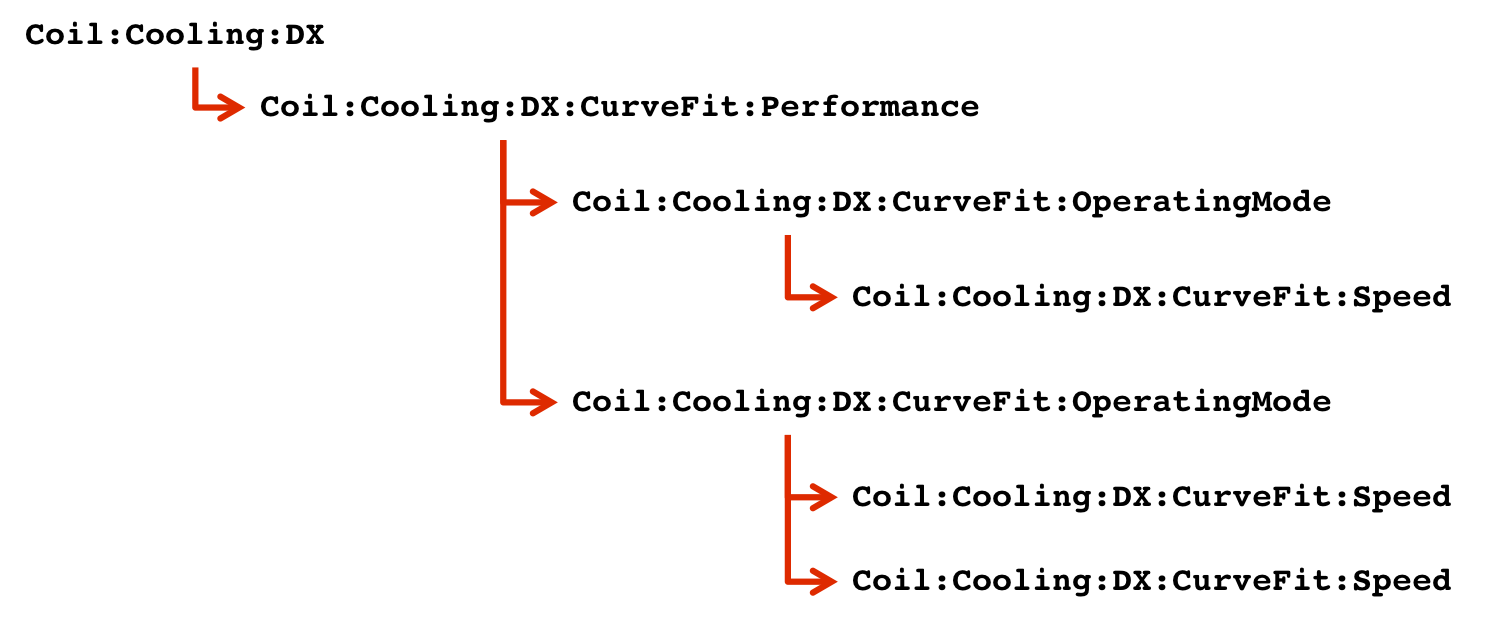
\includegraphics[width=0.9\textwidth, height=0.9\textheight, keepaspectratio=true]{media/cooling-coil-hierarchy.png}
\caption{Hierarchy of references between cooling coil objects \protect \label{fig:diagram-of-coil-object-references}}
\end{figure}

\subsubsection{Inputs}\label{inputs-01}

\paragraph{Field: Name}\label{field-name-01}

A unique user-assigned name for an instance of a cooling coil. Any reference to this cooling coil by another object will use this name.

\paragraph{Field: Evaporator Inlet Node Name}\label{field-evaporator-inlet-node-name-021}

The name of the HVAC system node from which the evaporator of the DX cooling coil draws its inlet air.

\paragraph{Field: Evaporator Outlet Node Name}\label{field-evaporator-outlet-node-name-021}

The name of the HVAC system node to which the evaporator of the DX cooling coil sends its outlet air.

\paragraph{Field: Availability Schedule Name}

The name of the schedule (ref: Schedule) that denotes whether the DX cooling coil can run during a given time period. A schedule value greater than 0 (usually 1 is used) indicates that the unit can be on during a given time period. A value less than or equal to 0 (usually 0 is used) denotes that the unit must be off. If this field is blank, the schedule has values of 1 for all time periods.

\paragraph{Field: Condenser Zone Name}\label{field-condenser-zone-name-6-001}

The name of a conditioned or unconditioned zone where the secondary coil (condenser) of DX system or a heat pump is to be placed. This is an optional input field specified only when user desires to reject the condenser heat into a zone. The heat rejected is modeled as internal sensible heat gain of the zone.

\paragraph{Field: Condenser Inlet Node Name}\label{field-condenser-inlet-node-name-6-001}

The name of the HVAC system node from which the condenser of the DX cooling coil draws its inlet air. If the condenser draws air from the outdoors, an \texttt{OutdoorAir:Node} object must be referenced.

\paragraph{Field: Condenser Outlet Node Name}\label{field-condenser-outlet-node-name-6-001}

The name of the HVAC system node to which the condenser of the DX cooling coil sends its outlet air.

\paragraph{Field: Performance Object Name}\label{field-performance-object-name-6-001}

The name of the Coil:Cooling:DX:CurveFit:Performance object that defines this coil's performance specifications.

\paragraph{Field: Condensate Collection Water Storage Tank Name}

This field is optional. It is used to describe where condensate from the coil is collected. If blank or omitted, then any coil condensate is discarded. Enter the name of a WaterUse:Storage object defined elsewhere and the condensate will then be collected in that tank.

\paragraph{Field: Evaporative Condenser Supply Water Storage Tank Name}\label{field-evaporative-condenser-supply-water-storage-tank-name-000}

This field is optional. It is used to describe where the coil obtains water used for evaporative cooling of its condenser. If blank or omitted, then the unit will obtain water directly from the mains. If the name of a WaterUse:Storage object is used here, then the unit will obtain its water from that tank. If a tank is specified, the unit will attempt to obtain all the water it uses from the tank. However, if the tank cannot provide all the water the condenser needs, then the unit will still operate and obtain the rest of the water it needs from the mains (referred to as StarvedWater).

\subsection{Coil:Cooling:DX:CurveFit:Performance}\label{coilcoolingdxcurvefitperformance}

This object defines basic unit control and other characteristics for one Coil:Cooling:DX object. For that Coil:Cooling:DX object, it also references one or more operating modes, which are defined using the Coil:Cooling:DX:CurveFit:OperatingMode object.

\subsubsection{Inputs}\label{inputs-02}

\paragraph{Field: Name}\label{field-name-02}

A unique user-assigned name for an instance of a cooling coil performance specification. Any reference to this cooling coil performance specification by a cooling coil object will use this name.

\paragraph{Field: Crankcase Heater Capacity}

This numeric field defines the crankcase heater capacity in Watts. When the outdoor air dry-bulb temperature is below the value specified in the input field Maximum Outdoor Dry-bulb Temperature for Crankcase Heater Operation (described below), the crankcase heater is enabled during the time that the compressor is not running. If this cooling coil is used as part of an air-to-air heat pump (Ref. AirLoopHVAC:UnitaryHeatPump:AirToAir or PackageTerminal: HeatPump:AirToAir), the crankcase heater defined for this DX cooling coil is ignored and the crankcase heater power defined for the DX heating coil (Ref. Coil:Heating:DX:SingleSpeed) is enabled during the time that the compressor is not running for either heating or cooling. The value for this input field must be greater than or equal to 0, and the default value is 0. To simulate a DX cooling coil without a crankcase heater, enter a value of 0.

\paragraph{Field: Minimum Outdoor Dry-Bulb Temperature for Compressor Operation}

This numeric field defines the minimum outdoor air dry-bulb temperature where the cooling coil compressor turns off. If this input field is left blank, the default value is -25 °C (-13 °F).

\paragraph{Field: Maximum Outdoor Dry-Bulb Temperature for Crankcase Heater Operation}

This numeric field defines the outdoor air dry-bulb temperature above which the compressor's crankcase heater is disabled. The value for this input field must be greater than or equal to 0.0 °C (32 °F), and the default value is 10 °C (50 °F).

\paragraph{Field: Unit Internal Static Air Pressure}

This field is to specify the internal static air pressure, in units of Pascals, associated with the unit s supply air flow for rating purposes. This field does not affect the performance during operation. The air pressure drop/rise input here should be internal in the sense that it is for the entire package of unitary equipment as it would be tested in a laboratory (including other non-cooling sections inside the package for filters, dampers, and or heating coils) but none of the external pressure drop for distributing supply air throughout the building. This is different from the input field called Pressure Rise in the fan object which includes both the external static pressure and the internal static pressure.
If this coil is used with a \hyperref[fanvariablevolume]{Fan:VariableVolume} to model a packaged variable-air-volume unit, then ratings for  EER, IEER, SEER, and Standard Rating (Net) Cooling Capacity will be calculated as defined ANSI/AHRI Standard 340/360 standard.  See also - the field "2017 Rated Evaporator Fan Power Per Volume Flow Rate" on the associated Coil:Cooling:DX:CurveFit:Speed object, which is also used to calculate the 2017 version of these standard ratings. The 2017 standard ratings are reported to the EIO file and to the predefined output table "2017 Standard Ratings for DX Coils."
Additionally, a newer definition for calculating EER, IEER, SEER2, and Standard Rating (Net) Cooling Capacity, was published in the 2022 version of AHRI 340-360.  These ratings are calculated using the value in the field "2023 Rated Evaporator Fan Power Per Volume Flow Rate"   The 2023 standard ratings are reported to the EIO file and to the predefined output table "2023 Standard Ratings for DX Coils" on the associated Coil:Cooling:DX:CurveFit:Speed object, which is also used to calculate the 2023 version of these standard ratings. The 2023 standard ratings are reported to the EIO file and to the predefined output table "2023 Standard Ratings for DX Coils."
This field is optional. If a value is provided, then it will be used, together with the associated fan characteristics when calculating standard ratings described above. If a value is not provided, then the standard ratings are still calculated, using values (user provided or default values) in the 'Rated Evaporator Fan Power Per Volume Flow Rate' fields, as described in those fields.

\paragraph{Field: Capacity Control Method}

This choice field defined the capacity control method. Valid choices for this input field are \textbf{Discrete} \textbf{Continuous}. The default for this field is \textbf{Discrete}. \textbf{Discrete} control mode allow the coil to operate at discrete speed levels. \textbf{Continuous} control mode allows the coil performance to be operated at continuously variable speeds.

\paragraph{Field: Evaporative Condenser Basin Heater Capacity}\label{field-evaporative-condenser-basin-heater-capacity-000}

This numeric field contains the capacity of the coil's electric evaporative cooler basin heater in Watts per degree Kelvin. This field only applies for Condenser Type = \textbf{EvaporativelyCooled}. This field is used in conjunction with the Evaporative Condenser Basin Heater Setpoint Temperature and Evaporative Condenser Basin Heater Operating Schedule Name described in the following fields. The basin heater electric power is equal to this field multiplied by the difference between the basin heater set point temperature and the outdoor dry-bulb temperature. The basin heater only operates when the DX coil is off, regardless of the basin heater schedule described below. The basin heater capacity must be greater than or equal to zero, with a default value of zero if this field is left blank.

\paragraph{Field: Evaporative Condenser Basin Heater Setpoint Temperature}\label{field-evaporative-condenser-basin-heater-setpoint-temperature-000}

This numeric field contains the set point temperature (\si{\celsius}) for the basin heater described in the previous field. This field only applies for Condenser Type = \textbf{EvaporativelyCooled}. The basin heater is active when the outdoor air dry-bulb temperature falls below this setpoint temperature, as long as the DX coil is off. This set point temperature must be greater than or equal to \SI{2}{\celsius} (\SI{35.6}{\fahrenheit}), and the default value is \SI{2}{\celsius} (\SI{35.6}{\fahrenheit}) if this field is left blank.

\paragraph{Field: Evaporative Condenser Basin Heater Operating Schedule Name}\label{field-evaporative-condenser-basin-heater-operating-schedule-name-000}

This alpha field contains the name of the basin heater operating schedule. This field only applies for Condenser Type = \textbf{EvaporativelyCooled}. The basin heater operating schedule is assumed to be an on/off schedule and the heater is available to operate any time the schedule value is greater than 0. The basin heater operates when scheduled on and the outdoor air dry-bulb temperature is below the set point temperature described in the previous field. If this field is left blank, the basin heater is available to operate throughout the simulation. Regardless of this schedule, the basin heater may only operate when the DX coil is off.

\paragraph{Field: Compressor Fuel Type}\label{field-compressor-fuel-type-000}

This alpha field determines the type of fuel that this cooling coil's compressor uses. This field has nine choices: \textbf{Electricity}, \textbf{NaturalGas}, \textbf{Propane}, \textbf{Diesel}, \textbf{Gasoline}, \textbf{FuelOilNo1}, \textbf{FuelOilNo2}, \textbf{OtherFuel1} and \textbf{OtherFuel2}. The default is \textbf{Electricity}.

\paragraph{Field: Base Operating Mode}\label{field-base-operating-mode}

The name corresponding to a Coil:Cooling:DX:CurveFit:OperatingMode object. Operating Mode is always used as the base design operating mode. This field is required.

\paragraph{Field: Alternate Operating Mode 1}\label{field-alternate-operating-mode-1}

The name corresponding to a Coil:Cooling:DX:CurveFit:OperatingMode object. Operating Mode is used as the alternate operating mode operating mode to be used for enhanced dehumidification when needed. If field is blank, the base operating mode will be used. This field is optional.

\paragraph{Field: Alternate Operating Mode 1}\label{field-alternate-operating-mode-2}

The name corresponding to a Coil:Cooling:DX:CurveFit:OperatingMode object. Operating Mode is used as to represent a reheat mode as a subcool reheat coil. If field is blank, the base operating mode will be used. This field is optional.

If there are 3 operating modes, it represents a subcool-reheat mode coil. The Operating Mode 1 represents a base operating mode coil. The Operating Mode 2 represents a subcool mode coil with lower SHR than the Operating Mode 1. The Operating Mode 3 represents a reheat mode coil with lower SHR than the Operating Mode 2. All 3 operation modes work together to represent a subcool reheat coil model. The operation procedure is described in \ref{coilcoolingdx}  

\paragraph{Field: Crankcase Heater Capacity Function of Temperature Curve Name}\label{outdoor-temperature-dependent-crankcase-heater-capacity-curve-name-0}

The name of a normalized Curve:* or Table:Lookup object encoding the
relationship between the crankcase heater capacity and the outdoor air
temperature. This curve can be any uni-variate curve or table. The output of
this curve is multiplied by the value in the field ``Crankcase Heater Capacity'.
If this field is missing or empty, constant crankcase heater capacity will be
assumed.

\subsection{Coil:Cooling:DX:CurveFit:OperatingMode}\label{coilcoolingdxcurvefitoperatingmode}

This object defines DX cooling coil performance for a single operating mode at rated conditions. Each operating mode may have one or more speeds, which are defined using the Coil:Cooling:DX:CurveFit:Speed object. Each operation mode can reference a maximum of 10 Coil:Cooling:DX:CurveFit:Speed objects.

\subsubsection{Inputs}\label{inputs-03}

\paragraph{Field: Name}\label{field-name-03}

A unique user-assigned name for an instance of a cooling coil operating mode. Any reference to this cooling coil operating mode by a cooling coil performance specification will use this name.

\paragraph{Field: Rated Gross Total Cooling Capacity}\label{field-rated-gross-total-cooling-capacity-1}

The total, full load gross cooling capacity (sensible plus latent) in Watts of the DX coil unit at rated conditions (air entering the cooling coil at 26.7 °C drybulb/19.4 °C wetbulb (80 °F drybulb/67 °F wetbulb), air entering the outdoor condenser coil at 35 °C drybulb/23.9 °C wetbulb (95 °F drybulb/75 °F wetbulb), and a cooling coil air flow rate defined by field rated air flow rate below). Capacity should be gross (i.e., the effect of supply air fan heat is NOT accounted for). When used in a heat pump, the gross rated total cooling capacity should be within 20\% of the gross rated heating capacity, otherwise a warning message is issued.

\paragraph{Field: Rated Evaporator Air Flow Rate}\label{field-rated-evaporator-air-flow-rate-2}

The air volume flow rate, in \si{\volumeFlowRate}, across the DX cooling coil evaporator section at rated conditions. The rated air volume flow rate should be between 0.00004027 m\(^{3}\)/s and 0.00006041 m\(^{3}\)/s per Watt of gross rated total cooling capacity (300 to 450 cfm/ton). For DOAS applications the rated air volume flow rate should be between 0.00001677 m\(^{3}\)/s and 0.00003355 m\(^{3}\)/s per watt of gross rated total cooling capacity (125 to 250 cfm/ton). The gross rated total cooling capacity, gross rated SHR and gross rated COP should be performance information for the unit with air entering the cooling coil at 26.7 °C drybulb/19.4 °C wetbulb (80 °F drybulb/67 °F wetbulb), air entering the outdoor condenser coil at 35 °C drybulb/23.9 °C wetbulb (95 °F drybulb/75 °F wetbulb), and the rated air volume flow rate defined here.

\paragraph{Field: Rated Condenser Air Flow Rate}\label{field-rated-condenser-air-flow-rate-2}

The air volume flow rate, in \si{\volumeFlowRate}, entering the evaporative condenser. This value is used to calculate the amount of water used to evaporatively cool the condenser inlet air. The minimum value for this field must be greater than zero, and this input field is autosizable (equivalent to 0.000144 m\(^{3}\)/s per watt of rated total cooling capacity {[}850 cfm/ton{]}). This field is not used when Condenser Type = \textbf{AirCooled}.

\paragraph{Field: Maximum Cycling Rate}

The maximum on-off cycling rate for the compressor (cycles per hour), which occurs at 50\% run time fraction. Suggested value is 3; zero value means latent degradation model is disabled. The default value for this field is zero. The supply air fan operating mode must be continuous (i.e., the supply air fan operating mode may be specified in other parent objects and is assumed continuous in some objects (e.g., CoilSystem:Cooling:DX) or can be scheduled in other objects (e.g., AirloopHVAC:UnitaryHeatCool); and this field, the previous two fields and the next field must have positive values in order to model latent capacity degradation.

\paragraph{Field: Ratio of Initial Moisture Evaporation Rate and Steady State Latent Capacity}

Ratio of the initial moisture evaporation rate from the cooling coil (when the compressor first turns off, in Watts) and the coil's steady-state latent capacity (Watts) at rated airflow and temperature conditions. Suggested value is 1.5; zero value means the latent degradation model is disabled. The default value for this field is zero. The supply air fan operating mode must be continuous (i.e., the supply air fan operating mode may be specified in other parent objects and is assumed continuous in some objects (e.g., CoilSystem:Cooling:DX) or can be scheduled in other objects (e.g., AirloopHVAC:UnitaryHeatCool); and this field, the previous field and the next two fields must have positive values in order to model latent capacity degradation.

\paragraph{Field: Latent Capacity Time Constant}

Time constant (in seconds) for the cooling coil's latent capacity to reach steady state after startup. Suggested value is 45: supply air fan operating mode must be continuous. That is, the supply air fan operating mode may be specified in other parent objects and is assumed continuous in some objects (e.g., CoilSystem:Cooling:DX) or can be scheduled in other objects (e.g., AirloopHVAC:UnitaryHeatCool).

\paragraph{Field: Nominal Time for Condensate Removal to Begin}

The nominal time (in seconds) after startup for condensate to begin leaving the coil's condensate drain line at the coil's rated airflow and temperature conditions, starting with a dry coil. Nominal time is equal to the ratio of the energy of the coil's maximum condensate holding capacity (J) to the coil's steady-state latent capacity (W). Suggested value is 1000; zero value means the latent degradation model is disabled. The default value for this field is zero. The supply air fan operating mode must be continuous (i.e., the supply air fan operating mode may be specified in other parent objects and is assumed continuous in some objects (e.g., CoilSystem:Cooling:DX) or can be scheduled in other objects (e.g., AirloopHVAC:UnitaryHeatCool), and this field as well as the previous three input fields for this object must have positive values in order to model latent capacity degradation.

\paragraph{Field: Apply Latent Degradation to Speeds Greater than 1}

This field determines whether latent capacity degradation is applied when the coil is operating at speeds greater than speed 1. The allowed choices are \textbf{Yes} or \textbf{No}, with the default being \textbf{No} if this field is left blank. Other input fields in this object allow the user to specify latent capacity degradation at each speed.

The latent capacity degradation model only applies when the ContinuousFanWithCyclingCompressor supply air fan operating mode is specified, to account for moisture evaporation from the wet cooling coil when the compressor cycles off but the supply air fan continues to operate. For the case of a single multi-speed compressor, latent capacity degradation may only be significant when the compressor cycles between speed 1 and off, but the losses may be extremely small when the compressor operates between speed 1 and speed 2 (or between speeds 2 and 3, etc.). In this case, the user may choose to specify \textbf{No} for this input field to neglect latent capacity degradation impacts at higher operating speeds. If latent capacity degradation is thought to be significant (e.g., intertwined or row-split cooling coil with multiple compressors feeding individual refrigerant circuits), then the user may choose to specify \textbf{Yes} and the latent capacity degradation model will be applied for speeds 2 through 10 as appropriate. The selection for this input field does not affect latent capacity degradation between speed 1 and off.

\paragraph{Field: Condenser Type}

The type of condenser used by the DX cooling coil. Valid choices for this input field are \textbf{AirCooled} or \textbf{EvaporativelyCooled}. The default for this field is \textbf{AirCooled}.

\paragraph{Field: Nominal Evaporative Condenser Pump Power}\label{field-nominal-evaporative-condenser-pump-power-1}

The rated power of the evaporative condenser water pump in Watts. This value is used to calculate the power required to pump the water used to evaporatively cool the condenser inlet air. The default value for this input field is zero, but it is autosizable (equivalent to 0.004266 W per watt {[}15 W/ton{]} of rated total cooling capacity). This field is not used when Condenser Type = \textbf{AirCooled}.

\paragraph{Field: Nominal Speed Number}\label{field-nominal-speed-number}

This numeric field specifies the speed number which corresponds to the rated capacity and air flow rates specified in this object. This value must be lower than or equal to the highest speed number defined below. If blank, defaults to the highest speed number used.

\paragraph{Field: Speed \textless{}x\textgreater{} Name}\label{field-speed-x-name}

For speed \textless{}x\textgreater{}, the name of the corresponding Coil:Cooling:DX:CurveFit:Speed object. Speed 1 is always used as the lowest speed. Speeds should be listed in ascending order from lowest capacity to highest capacity. Each coil operating mode may have up to 10 speeds defined.

\subsection{Coil:Cooling:DX:CurveFit:Speed}\label{coilcoolingdxcurvefitspeed}

This object defines DX cooling coil performance for a specific speed within a single operating mode. A speed can be used for a combination of air flow rates and capacities different than the rated air flow rates and capacities defined in Coil:Cooling:DX:CurveFit:OperatingMode. Each operating mode can reference a maximum of 10 speeds.

\subsubsection{Inputs}\label{inputs-04}

\paragraph{Field: Name}\label{field-name-04}

A unique user-assigned name for an instance of a cooling coil operating mode's speed. Any reference to a specific speed by a cooling coil operating mode will use this name.

\paragraph{Field: Gross Total Cooling Capacity Fraction}\label{field-gross-total-cooling-capacity-fraction}

This is the ratio of capacity at a specific speed to the operating mode's \textit{Rated Gross Total Cooling Capacity}. This field should be 1.0 for the \textit{Nominal Speed Number} specified in the Coil:Cooling:DX:CurveFit:OperatingMode object.

\paragraph{Field: Evaporator Air Flow Rate Fraction}\label{field-evaporator-air-flow-rate-fraction}

This is the ratio of evaporator air flow rate at a specific speed to the operating mode's \textit{Rated Evaporator Air Flow Rate}. This field should be 1.0 for the \textit{Nominal Speed Number} specified in the Coil:Cooling:DX:CurveFit:OperatingMode object.

\paragraph{Field: Condenser Air Flow Rate Fraction}\label{field-condenser-air-flow-rate-fraction}

This is the ratio of condenser air flow at a specific speed to the operating mode's \textit{Rated Condenser Air Flow Rate}. This field should be 1.0 for the \textit{Nominal Speed Number} specified in the Coil:Cooling:DX:CurveFit:OperatingMode object.

\paragraph{Field: Gross Sensible Heat Ratio}\label{field-gross-sensible-heat-ratio}

This numeric field defines the gross sensible heat ratio (sensible capacity divided by total cooling capacity) of the DX cooling coil at rated conditions for a specific speed. Both the sensible and total cooling capacities used should be gross (i.e., the effect of supply air fan heat is NOT accounted for).

\paragraph{Field: Gross Cooling COP}

The coefficient of performance is the ratio of the gross total cooling capacity in Watts to electrical power input in Watts of the DX cooling coil unit at rated conditions (air entering the cooling coil at 26.7 °C drybulb/19.4 °C wetbulb (80 °F drybulb/67 °F wetbulb), air entering the outdoor condenser coil at 35 °C drybulb/ 23.9 °C wetbulb (95 °F drybulb/75 °F wetbulb), and a cooling coil air flow rate defined by field rated air flow rate below). The input power includes electric power for the compressor(s) and condenser fan(s) but does not include the power consumption of the supply air fan. The gross COP should NOT account for the supply air fan. If this input field is left blank, the default value is 3.0.

\paragraph{Field: Active Fraction of Coil Face Area}\label{field-active-fraction-of-coil-face-area}

Defines the fraction of the cooling coil face which is actively cooled at a specific speed. Value varies between 0.0 and 1.0. For non-split-face coils, this should be 1.0.

\paragraph{Field: 2017 Rated Evaporator Fan Power Per Volume Flow Rate}

This field is the electric power for the evaporator (cooling coil) fan per air volume flow rate through the coil at the rated conditions in W/(m\(^{3}\)/s). The default value is 773.3 W/(m\(^{3}\)/s) (365 W/1000 cfm) if this field is left blank. If a value is entered, it must be \textgreater{}= 0.0 and \textless{}= 1250 W/(m\(^{3}\)/s). This value is only used to calculate the following metrics according to the 2017 version of ANSI/AHRI 210-240 standard: Seasonal Energy Efficiency Ratio (SEER), Energy Efficiency Ratio (EER), Integrated Energy Efficiency Ratio (IEER) and the Standard Rating (Net) Cooling Capacity.  These metrics will be outputs in the EnergyPlus eio file (ref. EnergyPlus Engineering Reference, 15.2 Coils) and also in the predefined tabular output reports (Output:Table:SummaryReports object, Equipment Summary). This value is not used for modeling the evaporator (cooling coil) fan during simulations; instead, it is used for calculating SEER, EER, IEER, and Standard Rating (Net) Cooling Capacity to assist the user in verifying their inputs for modeling this type of equipment. 
Note 1: Standard Ratings using this field will be reported in the "2017 Standard Ratings for DX Coils" table
Note 2: two values are calculated for SEER: 'SEER User' is calculated using user-input PLF curve and cooling coefficient of degradation; 'SEER Standard' is calculated using AHRI Std 210/240-2017 default PLF curve and cooling coefficient of degradation.
Note 3: SEER User, SEER Standard, EER, and IEER, and Standard Rating (Net) Cooling Capacity -- with cooling capacity less than 65,000 Btu/hr -- will be calculated according to ANSI/AHRI standard 210-240 (2017).
Note 4: EER, IEER, and Standard Rating (Net) Cooling Capacity -- with cooling capacity between 65,000 and 135,000 Btu/hr -- will be calculated according to ANSI/AHRI standard 340-360 (2013).

\paragraph{Field: 2023 Rated Evaporator Fan Power Per Volume Flow Rate}

This field is the electric power for the evaporator (cooling coil) fan per air volume flow rate through the coil at the rated conditions in W/(m\(^{3}\)/s). The default value is 934.4 W/(m3/s) (441 W/1000 cfm) if this field is left blank. If a value is entered, it must be \textgreater{}= 0.0 and \textless{}= 1505 W/(m\(^{3}\)/s). This value is only used to calculate the following metrics according to the 2023 version of ANSI/AHRI 210-240 standard: Seasonal Energy Efficiency Ratio (SEER2), Energy Efficiency Ratio (EER), Integrated Energy Efficiency Ratio (IEER) and the Standard Rating (Net) Cooling Capacity.  These metrics will be outputs in the EnergyPlus eio file (ref. EnergyPlus Engineering Reference, Section 15.2 Coils). This value is not used for modeling the evaporator (cooling coil) fan during simulations; instead, it is used for calculating SEER2, EER, IEER, and Standard Rating (Net) Cooling Capacity to assist the user in verifying their inputs for modeling this type of equipment. 
Note 1: Standard Ratings using this field will be reported in the "2023 Standard Ratings for DX Coils" table
Note 2: two values are calculated for SEER2. 'SEER2 User' is calculated using user-input PLF curve and cooling coefficient of degradation. 'SEER2 Standard' is calculated using AHRI Std 210/240-2023 default PLF curve and cooling coefficient of degradation.
Note 3: SEER2 User, SEER2 Standard, EER, IEER, and Standard Rating (Net) Cooling Capacity -- with cooling capacity less than 65,000 Btu/hr - will be calculated according to ANSI/AHRI standard 210-240 (2023).
Note 4: EER, IEER, and Standard Rating (Net) Cooling Capacity -- with cooling capacities between 65,000 and 135,000 Btu/hr -- will be calculated according to ANSI/AHRI standard 340-360 (2022).

\paragraph{Field: Evaporative Condenser Pump Power Fraction}\label{field-evaporative-condenser-pump-power-fraction}

The ratio of evaporative condenser pump power at a specific speed to the operating mode's \textit{Nominal Evaporative Condenser Pump Power}. This field is not used when Condenser Type = \textbf{AirCooled}.

\paragraph{Field: Evaporative Condenser Effectiveness}

The effectiveness of the evaporative condenser at a specific speed, which is used to determine the temperature of the air entering the outdoor condenser coil as follows:

\begin{equation}
Tcond,inlet = \,\left( {Twb,o} \right)\,\, + \,\,\left( {1 - EvapCondEffectivenes} \right)\left( {Tdb,o\,\, - Twb,o} \right)
\end{equation}

where

\emph{T\(_{cond,inlet}\)} = the temperature of the air entering the condenser coil (C)

\emph{T\(_{wb,o}\)} = the wet-bulb temperature of the outdoor air (C)

\emph{T\(_{db,o}\)} = the dry-bulb temperature of the outdoor air (C)

The resulting condenser inlet air temperature is used by the Total Cooling Capacity Modifier Function of Temperature Curve and the Energy Input Ratio Modifier Function of Temperature Curve. The default value for this field is 0.9, although valid entries can range from 0.0 to 1.0. This field is not used when Condenser Type = \textbf{AirCooled}.

If the user wants to model an air-cooled condenser, they should simply specify \textbf{AirCooled} in the field \textit{Condenser Type}. In this case, the Total Cooling Capacity Modifier Function of Temperature Curve and the Energy Input Ratio Modifier Function of Temperature Curve input fields for this object should reference performance curves that are a function of outdoor dry-bulb temperature.

If the user wishes to model an evaporative-cooled condenser AND they have performance curves that are a function of the wet-bulb temperature of air entering the condenser coil, then the user should specify Condenser Type = \textbf{EvaporativelyCooled} and the evaporative condenser effectiveness value should be entered as 1.0. In this case, the Total Cooling Capacity Modifier Function of Temperature Curve and the Energy Input Ratio Modifier Function of Temperature Curve input fields for this object should reference performance curves that are a function of the wet-bulb temperature of air entering the condenser coil.

If the user wishes to model an air-cooled condenser that has evaporative media placed in front of it to cool the air entering the condenser coil, then the user should specify Condenser Type = \textbf{EvaporativelyCooled}. The user must also enter the appropriate evaporative effectiveness for the media. In this case, the Total Cooling Capacity Modifier Function of Temperature Curve and the Energy Input Ratio Modifier Function of Temperature Curve input fields for this object should reference performance curves that are a function of outdoor dry-bulb temperature. Be aware that the evaporative media will significantly reduce the dry-bulb temperature of the air entering the condenser coil, so the Total Cooling Capacity and EIR Modifier Function of Air Flow Fraction Curves must be valid for the expected range of dry-bulb temperatures that will be entering the condenser coil.

\paragraph{Field: Total Cooling Capacity Modifier Function of Temperature Curve Name}

The name of a bivariate (e.g. biquadratic) or univariate (e.g. quadratic) curve or table object (ref Curve:* and Table:*) that parameterizes the variation of the gross total cooling capacity for a specific speed as a function of the wet-bulb temperature of the air entering the evaporator section, and the dry-bulb temperature of the air entering the condenser section (wet-bulb temperature if modeling an evaporative-cooled condenser). If a univariate curve or table is specified, then the independent variable is the entering condenser temperature. The curve is normalized to 1 at 19.44 °C (67 °F) indoor wet-bulb temperature and 35 °C (95 °F) outdoor dry-bulb temperature. The output of this curve is multiplied by the operating mode's \textit{Rated Gross Total Cooling Capacity} to give the gross total cooling capacity at specific temperature operating conditions (i.e., at temperatures different from the rating point temperatures). The curve is normalized to have the value of 1.0 at the rating point.

\paragraph{Field: Total Cooling Capacity Modifier Function of Air Flow Fraction Curve Name}\label{field-total-cooling-capacity-function-of-air-flow-fraction-curve-name}

The name of a univariate (e.g. quadratic) curve or table object (ref Curve:* and Table:*) that parameterizes the variation of the gross total cooling capacity for a specific speed as a function of the ratio of actual air flow rate across the cooling coil to the rated air flow rate for a specific speed (i.e., fraction of full load flow). The output of this curve is multiplied by the operating mode's \textit{Rated Gross Total Cooling Capacity} and the total cooling capacity modifier curve (function of temperature) to give the gross total cooling capacity for a specific speed at the specific temperature and air flow conditions at which the coil is operating. The curve is normalized to have the value of 1.0 when the actual air flow rate equals the rated air flow rate for Speed \textless{}x\textgreater{}.

\paragraph{Field: Energy Input Ratio Modifier Function of Temperature Curve Name}

The name of a bivariate (e.g. biquadratic) curve or table object (ref Curve:* and Table:*) that parameterizes the variation of the energy input ratio (EIR) for a specific speed as a function of the wetbulb temperature of the air entering the evaporator section and the drybulb temperature of the air entering the condenser section (wetbulb temperature if modeling an evaporative-cooled condenser). The curve is normalized to 1 at 19.44 °C (67 °F) indoor wet-bulb temperature and 35 °C (95 °F) outdoor dry-bulb temperature. The EIR is the inverse of the COP. The output of this curve is multiplied by the rated EIR for a specific speed (inverse of rated COP for a specific speed) to give the EIR for a specific speed at specific temperature operating conditions (i.e., at temperatures different from the rating point temperatures).

\paragraph{Field: Energy Input Ratio Modifier Function of Air Flow Fraction Curve Name}\label{field-energy-input-ratio-function-of-air-flow-fraction-curve-name}

The name of a univariate (e.g. quadratic) curve or table object (ref Curve:* and Table:*) that parameterizes the variation of the energy input ratio (EIR) for a specific speed as a function of the ratio of actual air flow rate across the cooling coil to the rated air flow rate for a specific speed (i.e., fraction of full load flow). The EIR is the inverse of the COP. The output of this curve is multiplied by the rated EIR and the EIR modifier curve (function of temperature) to give the EIR for a specific speed at the specific temperature and air flow conditions at which the cooling coil is operating. This curve is normalized to a value of 1.0 when the actual air flow rate equals the rated air flow rate for a specific speed.

\paragraph{Field: Part Load Fraction Correlation Curve Name}

The name of a univariate (e.g. quadratic) curve or table object (ref Curve:* and Table:*) that parameterizes the variation of electrical power input to the DX unit as a function of the part load ratio (PLR, sensible cooling load/steady-state sensible cooling capacity for a specific speed). The product of the rated EIR and EIR modifier curves is divided by the output of this curve to give the effective EIR for a given simulation timestep for a specific speed. The part load fraction (PLF) correlation accounts for efficiency losses due to compressor cycling.

The part load fraction correlation should be normalized to a value of 1.0 when the part load ratio equals 1.0 (i.e., no efficiency losses when the compressor(s) run continuously for the simulation timestep). For PLR values between 0 and 1 (0 \textless{} = PLR \textless{} 1), the following rules apply:

\begin{lstlisting}
       PLF > = 0.7     and     PLF > = PLR
\end{lstlisting}

If PLF \textless{} 0.7 a warning message is issued, the program resets the PLF value to 0.7, and the simulation proceeds. The runtime fraction of the coil is defined as PLR/PLF. If PLF \textless{} PLR, then a warning message is issued and the runtime fraction of the coil is limited to 1.0.

A typical part load fraction correlation for a conventional DX cooling coil (a specific speed) would be:

\begin{lstlisting}
       PLF = 0.85 + 0.15(PLR)
\end{lstlisting}

If the user wishes to model no efficiency degradation due to compressor cycling, the part load fraction correlation should be defined as follows:

\begin{lstlisting}
       PLF = 1.0 + 0.0(PLR)
\end{lstlisting}

\paragraph{Field: Rated Waste Heat Fraction of Power Input}\label{field-rated-waste-heat-fraction-of-power-input}

The fraction of energy input to the cooling coil that is available as recoverable waste heat at full load and rated conditions for a specific speed.

\paragraph{Field: Waste Heat Modifier Function of Temperature Curve Name}\label{field-waste-heat-function-of-temperature-curve-name}

The name of a bivariate (e.g. biquadratic) curve or table object (ref Curve:* and Table:*) that parameterizes the variation of the waste heat recovery as a function of outdoor dry-bulb temperature and the entering coil dry-bulb temperature at a specific speed. The output of this curve is multiplied by the rated waste heat fraction at specific temperature operating conditions (i.e., at temperatures different from the rating point). The curve is normalized to a value of 1.0 at the rating point. When the fuel type is electricity, this field can remain blank since it is ignored by the program in this instance. When the fuel type is not electricity and the parent object AirLoopHVAC:UnitaryHeatPump:AirToAir:MultiSpeed does not require waste heat calculations, this field is ignored. If the field is blank, a warning will be issued and simulation continues. When the fuel type is not electricity and the parent object AirLoopHVAC:UnitaryHeatPump:AirToAir:MultiSpeed requires waste heat calculations, if this field is left blank, the program assumes a constant value of 1 to make simulation continue and a warning will be issued.

\paragraph{Field: Sensible Heat Ratio Modifier Function of Temperature Curve Name}

The name of a bivariate (e.g. biquadratic) curve or table object (ref Curve:* and Table:*) that parameterizes the variation of the sensible heat ratio (SHR) as a function of DX cooling coil entering air wet-bulb and dry-bulb temperatures. The output of this curve is multiplied by the rated SHR and the SHR modifier curve (function of flow fraction) to give the SHR at the specific coil entering air temperature and air flow conditions at which the cooling coil is operating. This curve is normalized to a value of 1.0 at the rated condition. This input field is optional. If this input is not blank then the \textit{Sensible Heat Ratio Modifier Function of Flow Fraction Curve Name} must also be entered. If left blank, SHR is calculated using the apparatus dew point method based on total capacity and coil bypass factor.

\paragraph{Field: Sensible Heat Ratio Modifier Function of Flow Fraction Curve Name}

The name of a univariate (e.g. quadratic) curve or table object (ref Curve:* and Table:*) that parameterizes the variation of the sensible heat ratio (SHR) as a function of the ratio of actual air flow rate across the cooling coil to the rated air flow rate (i.e., fraction of full load flow). The output of this curve is multiplied by the rated SHR and the SHR modifier curve (function of temperature) to give the SHR at the specific temperature and air flow conditions at which the cooling coil is operating. This curve is normalized to a value of 1.0 when the actual air flow rate equals the rated air flow rate. This input field is optional. If this input is not blank then the \textit{Sensible Heat Ratio Modifier Function of Temperature Curve Name} must also be entered. If left blank, SHR is calculated using the apparatus dew point method based on total capacity and coil bypass factor.

Following is an example input for a single-speed air-cooled cooling DX coil.

\begin{lstlisting}

Coil:Cooling:DX,
  Single Speed Cooling Coil,          !- Name
  Cooling Coil Air Inlet Node,        !- Evaporator Inlet Node Name
  Cooling Coil Air Outlet Node,       !- Evaporator Outlet Node Name
  FanAndCoilAvailSched,               !- Availability Schedule Name
  ,                                   !- Condenser Zone Name
  Outdoor Condenser Air Inlet Node,   !- Condenser Inlet Node Name
  Outdoor Condenser Air Outlet Node,  !- Condenser Outlet Node Name
  Single Speed Cooling Coil Performance, !- Performance Object Name
  , !- Condensate Collection Water Storage Tank Name
  ; !- Evaporative Condenser Supply Water Storage Tank Name

Coil:Cooling:DX:CurveFit:Performance,
  Single Speed Cooling Coil Performance,  !- Name
  0.0,       !- Crankcase Heater Capacity {W}
  -25.0,     !- Minimum Outdoor Dry-Bulb Temperature for Compressor Operation {C}
  10.0,      !- Maximum Outdoor Dry-Bulb Temperature for Crankcase Heater Operation {C}
  500.0,     !- Unit Internal Static Air Pressure {Pa}
  Discrete,  !- Capacity Control Method
  ,          !- Evaporative Condenser Basin Heater Capacity {W}
  ,          !- Evaporative Condenser Basin Heater Setpoint Temperature {C}
  ,          !- Evaporative Condenser Basin Heater Operating Schedule Name
  Electricity,   !- Compressor Fuel Type
  Single Speed Cooling Coil Operating Mode; !- Operating Mode 1 Name

Coil:Cooling:DX:CurveFit:OperatingMode,
  Single Speed Cooling Coil Operating Mode, !-  Name
  Autosize,  !- Rated Gross Total Cooling Capacity {W}
  Autosize,  !- Rated Evaporator Air Flow Rate {m3/s}
  ,          !- Rated Condenser Air Flow Rate {m3/s}
  0.0,       !- Maximum Cycling Rate {cycles/hr}
  0.0,       !- Ratio of Initial Moisture Evaporation Rate and Steady State Latent Capacity
  0.0,       !- Latent Capacity Time Constant {s}
  0.0,       !- Nominal Time for Condensate Removal to Begin {s}
  No,        !- Apply Latent Degradation to Speeds Greater than 1
  AirCooled, !- Condenser Type
  1,         !- Nominal Speed Number
  Single Speed Cooling Coil Speed 1;  !- Speed 1 Name

Coil:Cooling:DX:CurveFit:Speed,
  Single Speed Cooling Coil Speed 1,  !- Name
  1.0,                                !- Gross Total Cooling Capacity Fraction
  1.0,                                !- Evaporator Air Flow Rate Fraction
  1.0,                                !- Condenser Air Flow Rate Fraction
  Autosize,                           !- Gross Sensible Heat Ratio
  3.0,                                !- Gross Cooling COP
  1.0,                                !- Active Fraction of Coil Face Area
  773.3,                              !- 2017 Rated Evaporator Fan Power Per Volume Flow Rate {W/(m3/s)}
  934.4,                              !- 2023 Rated Evaporator Fan Power Per Volume Flow Rate {W/(m3/s)}
  1.0,                                !- Evaporative Condenser Pump Power Fraction
  0.9,                                !- Evaporative Condenser Effectiveness
  Single Speed Cool Cap fTemp,        !- Total Cooling Capacity Modifier Function of Temperature Curve Name
  Single Speed Cool Cap fFlow,        !- Total Cooling Capacity Modifier Function of Air Flow Fraction Curve Name
  Single Speed Cool EIR fTemp,        !- Energy Input Ratio Modifier Function of Temperature Curve Name
  Single Speed Cool EIR fFlow,        !- Energy Input Ratio Modifier Function of Air Flow Fraction Curve Name
  Single Speed Cool fPLR,             !- Part Load Fraction Correlation Curve Name
  0.2,                                !- Rated Waste Heat Fraction of Power Input
  Single Speed Waste Heat fTemp;      !- Waste Heat Function of Temperature Curve Name
  ,                                   !- Sensible Heat Ratio Modifier Function of Temperature Curve Name
  ;                                   !- Sensible Heat Ratio Modifier Function of Flow Fraction Curve Name

\end{lstlisting}

Following is an example input for a three-speed evaporatively-cooled cooling DX coil.

\begin{lstlisting}

Coil:Cooling:DX,
  Three Speed Cooling Coil,     !- Name
  Cooling Coil Air Inlet Node,  !- Evaporator Inlet Node Name
  Cooling Coil Air Outlet Node, !- Evaporator Outlet Node Name
  FanAndCoilAvailSched,         !- Availability Schedule Name
  ,                             !- Condenser Zone Name
  Outdoor Condenser Air Inlet Node,   !- Condenser Inlet Node Name
  Outdoor Condenser Air Outlet Node,  !- Condenser Outlet Node Name
  Three Speed Cooling Coil Performance,   !- Performance Object Name
  , !- Condensate Collection Water Storage Tank Name
  ; !- Evaporative Condenser Supply Water Storage Tank Name

Coil:Cooling:DX:CurveFit:Performance,
  Three Speed Cooling Coil Performance,   !- Name
  0.0,       !- Crankcase Heater Capacity {W}
  -25.0,     !- Minimum Outdoor Dry-Bulb Temperature for Compressor Operation {C}
  10.0,      !- Maximum Outdoor Dry-Bulb Temperature for Crankcase Heater Operation {C}
  500.0,     !- Unit Internal Static Air Pressure {Pa}
  Discrete,  !- Capacity Control Method
  0.0,       !- Evaporative Condenser Basin Heater Capacity {W}
  2.0,       !- Evaporative Condenser Basin Heater Setpoint Temperature {C}
  FanAndCoilAvailSched, !- Evaporative Condenser Basin Heater Operating Schedule Name
  Electricity,          !- Compressor Fuel Type
  Three Speed Cooling Coil Operating Mode;  !- Operating Mode 1 Name

Coil:Cooling:DX:CurveFit:OperatingMode,
  Three Speed Cooling Coil Operating Mode,  !-  Name
  Autosize,  !- Rated Gross Total Cooling Capacity {W}
  Autosize,  !- Rated Evaporator Air Flow Rate {m3/s}
  Autosize,  !- Rated Condenser Air Flow Rate {m3/s}
  0.0,       !- Maximum Cycling Rate {cycles/hr}
  0.0,       !- Ratio of Initial Moisture Evaporation Rate and Steady State Latent Capacity
  0.0,       !- Latent Capacity Time Constant {s}
  0.0,       !- Nominal Time for Condensate Removal to Begin {s}
  No,        !- Apply Latent Degradation to Speeds Greater than 1
  Aircooled, !- Condenser Type
  ,          !- Nominal Evaporative Condenser Pump Power
  Three Speed Cooling Coil Speed 1,  !- Speed 1 Name
  Three Speed Cooling Coil Speed 2,  !- Speed 2 Name
  Three Speed Cooling Coil Speed 3;  !- Speed 3 Name

Coil:Cooling:DX:CurveFit:Speed,
  Three Speed Cooling Coil Speed 1, !- Name
  0.4,       !- Gross Total Cooling Capacity Fraction
  0.4,       !- Evaporator Air Flow Rate Fraction
  0.4,       !- Condenser Air Flow Rate Fraction
  Autosize,  !- Gross Sensible Heat Ratio
  4.5,       !- Gross Cooling COP
  1.0,       !- Active Fraction of Coil Face Area
  453.3,     !- Rated Evaporator Fan Power Per Volume Flow Rate {W/(m3/s)}
  0.4,       !- Evaporative Condenser Pump Power Fraction
  0.9,       !- Evaporative Condenser Effectiveness
  Three Speed Cool Cap fTemp Spd 1, !- Total Cooling Capacity Modifier Function of Temperature Curve Name
  Three Speed Cool Cap fFlow Spd 1, !- Total Cooling Capacity Modifier Function of Air Flow Fraction Curve Name
  Three Speed Cool EIR fTemp Spd 1, !- Energy Input Ratio Modifier Function of Temperature Curve Name
  Three Speed Cool EIR fFlow Spd 1, !- Energy Input Ratio Modifier Function of Air Flow Fraction Curve Name
  Three Speed Cool fPLR Spd 1,      !- Part Load Fraction Correlation Curve Name
  0.2,                              !- Rated Waste Heat Fraction of Power Input
  Three Speed Waste Heat fTemp Spd 1, !- Waste Heat Function of Temperature Curve Name
  Three Speed SHR fTemp Spd 1, !- Sensible Heat Ratio Modifier Function of Temperature Curve Name
  Three Speed SHR fFlow Spd 1; !- Sensible Heat Ratio Modifier Function of Flow Fraction Curve Name

Coil:Cooling:DX:CurveFit:Speed,
  Three Speed Cooling Coil Speed 2, !- Name
  0.7,       !- Gross Total Cooling Capacity Fraction
  0.7,       !- Evaporator Air Flow Rate Fraction
  0.7,       !- Condenser Air Flow Rate Fraction
  Autosize,  !- Gross Sensible Heat Ratio
  3.5,       !- Gross Cooling COP
  1.0,       !- Active Fraction of Coil Face Area
  613.3,     !- Rated Evaporator Fan Power Per Volume Flow Rate {W/(m3/s)}
  0.7,       !- Evaporative Condenser Pump Power Fraction
  0.9,       !- Evaporative Condenser Effectiveness
  Three Speed Cool Cap fTemp Spd 2, !- Total Cooling Capacity Modifier Function of Temperature Curve Name
  Three Speed Cool Cap fFlow Spd 2, !- Total Cooling Capacity Modifier Function of Air Flow Fraction Curve Name
  Three Speed Cool EIR fTemp Spd 2, !- Energy Input Ratio Modifier Function of Temperature Curve Name
  Three Speed Cool EIR fFlow Spd 2, !- Energy Input Ratio Modifier Function of Air Flow Fraction Curve Name
  Three Speed Cool fPLR Spd 2,      !- Part Load Fraction Correlation Curve Name
  0.2, !- Rated Waste Heat Fraction of Power Input
  Three Speed Waste Heat fTemp Spd 2, !- Waste Heat Function of Temperature Curve Name
  Three Speed SHR fTemp Spd 2, !- Sensible Heat Ratio Modifier Function of Temperature Curve Name
  Three Speed SHR fFlow Spd 2; !- Sensible Heat Ratio Modifier Function of Flow Fraction Curve Name

Coil:Cooling:DX:CurveFit:Speed,
  Three Speed Cooling Coil Speed 3, !- Name
  1.0,      !- Gross Total Cooling Capacity Fraction
  1.0,      !- Evaporator Air Flow Rate Fraction
  1.0,      !- Condenser Air Flow Rate Fraction
  Autosize, !- Gross Sensible Heat Ratio
  3.0,      !- Gross Cooling COP
  1.0,      !- Active Fraction of Coil Face Area
  773.3,    !- Rated Evaporator Fan Power Per Volume Flow Rate {W/(m3/s)}
  1.0,      !- Evaporative Condenser Pump Power Fraction
  0.9,      !- Evaporative Condenser Effectiveness
  Three Speed Cool Cap fTemp Spd 3, !- Total Cooling Capacity Modifier Function of Temperature Curve Name
  Three Speed Cool Cap fFlow Spd 3, !- Total Cooling Capacity Modifier Function of Air Flow Fraction Curve Name
  Three Speed Cool EIR fTemp Spd 3, !- Energy Input Ratio Modifier Function of Temperature Curve Name
  Three Speed Cool EIR fFlow Spd 3, !- Energy Input Ratio Modifier Function of Air Flow Fraction Curve Name
  Three Speed Cool fPLR Spd 3,      !- Part Load Fraction Correlation Curve Name
  0.2, !- Rated Waste Heat Fraction of Power Input
  Three Speed Waste Heat fTemp Spd 3, !- Waste Heat Function of Temperature Curve Name
  Three Speed SHR fTemp Spd 3, !- Sensible Heat Ratio Modifier Function of Temperature Curve Name

\end{lstlisting}

Following is an example input for a single cooling DX coil with 3 operation modes as normal, subcool and reheat to represent a subcool reheat coil model.

\begin{lstlisting}

  Coil:Cooling:DX,
    Sys 1 Furnace DX Cool Cooling Coil,  !- Name
    Sys 1 Furnace DX Cool Supply Fan Outlet,  !- Evaporator Inlet Node Name
    Sys 1 Furnace DX Cool Cooling Coil Outlet,  !- Evaporator Outlet Node Name
    ,                        !- Availability Schedule Name
    ,                        !- Condenser Zone Name
    Sys 1 Furnace DX Cool Cooling Coil Condenser Inlet,  !- Condenser Inlet Node Name
    Sys 1 Furnace DX Cool Cooling Coil Condenser Outlet Node,  !- Condenser Outlet Node Name
    Sys 1 Furnace DX Cool Cooling Coil Performance,  !- Performance Object Name
    ,                        !- Condensate Collection Water Storage Tank Name
    ;                        !- Evaporative Condenser Supply Water Storage Tank Name

  Coil:Cooling:DX:CurveFit:Performance,
    Sys 1 Furnace DX Cool Cooling Coil Performance,  !- Name
    0,                       !- Crankcase Heater Capacity {W}
    ,                        !- Minimum Outdoor Dry-Bulb Temperature for Compressor Operation {C}
    10,                      !- Maximum Outdoor Dry-Bulb Temperature for Crankcase Heater Operation {C}
    ,                        !- Unit Internal Static Air Pressure {Pa}
    ,                        !- Capacity Control Method
    ,                        !- Evaporative Condenser Basin Heater Capacity {W/K}
    ,                        !- Evaporative Condenser Basin Heater Setpoint Temperature {C}
    ,                        !- Evaporative Condenser Basin Heater Operating Schedule Name
    Electricity,             !- Compressor Fuel Type
    Sys 1 Furnace DX Cool Cooling Coil Operating Mode,  !- Base Operating Mode
    Sys 1 Furnace DX Cool Cooling Coil Alternative Mode 1,  !- Alternative Operating Mode 1
    Sys 1 Furnace DX Cool Cooling Coil Alternative Mode 2;  !- Alternative Operating Mode 1

  Coil:Cooling:DX:CurveFit:OperatingMode,
    Sys 1 Furnace DX Cool Cooling Coil Operating Mode,  !- Name
    autosize,                !- Rated Gross Total Cooling Capacity {W}
    autosize,                !- Rated Evaporator Air Flow Rate {m3/s}
    ,                        !- Rated Condenser Air Flow Rate {m3/s}
    0,                       !- Maximum Cycling Rate {cycles/hr}
    0,                       !- Ratio of Initial Moisture Evaporation Rate and Steady State Latent Capacity {dimensionless}
    0,                       !- Latent Capacity Time Constant {s}
    0,                       !- Nominal Time for Condensate Removal to Begin {s}
    ,                        !- Apply Latent Degradation to Speeds Greater than 1
    AirCooled,               !- Condenser Type
    0,                       !- Nominal Evaporative Condenser Pump Power {W}
    1,                       !- Nominal Speed Number
    Sys 1 Furnace DX Cool Cooling Coil Speed 1 Performance;  !- Speed 1 Name

  Coil:Cooling:DX:CurveFit:Speed,
    Sys 1 Furnace DX Cool Cooling Coil Speed 1 Performance,  !- Name
    1.0,                     !- Gross Total Cooling Capacity Fraction
    1.0,                     !- Evaporator Air Flow Rate Fraction
    1.0,                     !- Condenser Air Flow Rate Fraction
    0.77,                !- Gross Sensible Heat Ratio
    4.17,                       !- Gross Cooling COP {W/W}
    1.0,                     !- Active Fraction of Coil Face Area
    ,                        !- Rated Evaporator Fan Power Per Volume Flow Rate {W/(m3/s)}
    1.0,                     !- Evaporative Condenser Pump Power Fraction
    0,                       !- Evaporative Condenser Effectiveness {dimensionless}
    NormalTempCoolingCAPFTemp,  !- Total Cooling Capacity Modifier Function of Temperature Curve Name
    NormalFlowCoolingCAPFFF,  !- Total Cooling Capacity Modifier Function of Air Flow Fraction Curve Name
    NormalTempCoolingEIRFTemp,  !- Energy Input Ratio Modifier Function of Temperature Curve Name
    NormalFlowCoolingEIRFFF,  !- Energy Input Ratio Modifier Function of Air Flow Fraction Curve Name
    Sys 1 Furnace DX Cool Cool Coil PLF,  !- Part Load Fraction Correlation Curve Name
    ,                        !- Rated Waste Heat Fraction of Power Input {dimensionless}
    ,                        !- Waste Heat Modifier Function of Temperature Curve Name
    NormalSHRTempCoolingFFF,  !- Sensible Heat Ratio Modifier Function of Temperature Curve Name
    NormalSHRFlowCoolingFFF;  !- Sensible Heat Ratio Modifier Function of Flow Fraction Curve Name

  Coil:Cooling:DX:CurveFit:OperatingMode,
    Sys 1 Furnace DX Cool Cooling Coil Alternative Mode 1,  !- Name
    autosize,                !- Rated Gross Total Cooling Capacity {W}
    autosize,                !- Rated Evaporator Air Flow Rate {m3/s}
    ,                        !- Rated Condenser Air Flow Rate {m3/s}
    0,                       !- Maximum Cycling Rate {cycles/hr}
    0,                       !- Ratio of Initial Moisture Evaporation Rate and Steady State Latent Capacity {dimensionless}
    0,                       !- Latent Capacity Time Constant {s}
    0,                       !- Nominal Time for Condensate Removal to Begin {s}
    ,                        !- Apply Latent Degradation to Speeds Greater than 1
    AirCooled,               !- Condenser Type
    0,                       !- Nominal Evaporative Condenser Pump Power {W}
    1,                       !- Nominal Speed Number
    Sys 1 Furnace DX Cool Cooling Coil Alternative Mode 1 Performance;  !- Speed 1 Name

  Coil:Cooling:DX:CurveFit:Speed,
    Sys 1 Furnace DX Cool Cooling Coil Alternative Mode 1 Performance,  !- Name
    1.0,                     !- Gross Total Cooling Capacity Fraction
    1.0,                     !- Evaporator Air Flow Rate Fraction
    1.0,                     !- Condenser Air Flow Rate Fraction
    0.66,                !- Gross Sensible Heat Ratio
    4.10,                       !- Gross Cooling COP {W/W}
    1.0,                     !- Active Fraction of Coil Face Area
    ,                        !- Rated Evaporator Fan Power Per Volume Flow Rate {W/(m3/s)}
    1.0,                     !- Evaporative Condenser Pump Power Fraction
    0,                       !- Evaporative Condenser Effectiveness {dimensionless}
    SubcoolTempCoolingCAPFTemp,  !- Total Cooling Capacity Modifier Function of Temperature Curve Name
    SubcoolFlowCoolingCAPFFF,  !- Total Cooling Capacity Modifier Function of Air Flow Fraction Curve Name
    SubcoolTempCoolingEIRFTemp,  !- Energy Input Ratio Modifier Function of Temperature Curve Name
    SubcoolFlowCoolingEIRFFF,  !- Energy Input Ratio Modifier Function of Air Flow Fraction Curve Name
    Sys 1 Furnace DX Cool Cool Coil PLF,  !- Part Load Fraction Correlation Curve Name
    ,                        !- Rated Waste Heat Fraction of Power Input {dimensionless}
    ,                        !- Waste Heat Modifier Function of Temperature Curve Name
    SubcoolSHRTempCoolingCAPFTemp,   !- Sensible Heat Ratio Modifier Function of Temperature Curve Name
    SubcoolSHRFlowCoolingCAPFFF;     !- Sensible Heat Ratio Modifier Function of Flow Fraction Curve Name

  Coil:Cooling:DX:CurveFit:OperatingMode,
    Sys 1 Furnace DX Cool Cooling Coil Alternative Mode 2,  !- Name
    autosize,                !- Rated Gross Total Cooling Capacity {W}
    autosize,                !- Rated Evaporator Air Flow Rate {m3/s}
    ,                        !- Rated Condenser Air Flow Rate {m3/s}
    0,                       !- Maximum Cycling Rate {cycles/hr}
    0,                       !- Ratio of Initial Moisture Evaporation Rate and Steady State Latent Capacity {dimensionless}
    0,                       !- Latent Capacity Time Constant {s}
    0,                       !- Nominal Time for Condensate Removal to Begin {s}
    ,                        !- Apply Latent Degradation to Speeds Greater than 1
    AirCooled,               !- Condenser Type
    0,                       !- Nominal Evaporative Condenser Pump Power {W}
    1,                       !- Nominal Speed Number
    Sys 1 Furnace DX Cool Cooling Coil Alternative Mode 2 Performance;  !- Speed 1 Name

  Coil:Cooling:DX:CurveFit:Speed,
    Sys 1 Furnace DX Cool Cooling Coil Alternative Mode 2 Performance,  !- Name
    1.0,                     !- Gross Total Cooling Capacity Fraction
    1.0,                     !- Evaporator Air Flow Rate Fraction
    1.0,                     !- Condenser Air Flow Rate Fraction
    0.16,                !- Gross Sensible Heat Ratio
    1.41,                       !- Gross Cooling COP {W/W}
    1.0,                     !- Active Fraction of Coil Face Area
    ,                        !- Rated Evaporator Fan Power Per Volume Flow Rate {W/(m3/s)}
    1.0,                     !- Evaporative Condenser Pump Power Fraction
    0,                       !- Evaporative Condenser Effectiveness {dimensionless}
    ReheatTempCoolingCAPFTemp,  !- Total Cooling Capacity Modifier Function of Temperature Curve Name
    ReheatFlowCoolingCAPFFF,  !- Total Cooling Capacity Modifier Function of Air Flow Fraction Curve Name
    ReheatTempCoolingEIRFTemp,  !- Energy Input Ratio Modifier Function of Temperature Curve Name
    ReheatFlowCoolingEIRFFF,  !- Energy Input Ratio Modifier Function of Air Flow Fraction Curve Name
    Sys 1 Furnace DX Cool Cool Coil PLF,  !- Part Load Fraction Correlation Curve Name
    ,                        !- Rated Waste Heat Fraction of Power Input {dimensionless}
    ,                        !- Waste Heat Modifier Function of Temperature Curve Name
    ReheatSHRTempCoolingCAPFTemp,  !- Sensible Heat Ratio Modifier Function of Temperature Curve Name
    ReheatSHRFlowCoolingCAPFFF;    !- Sensible Heat Ratio Modifier Function of Flow Fraction Curve Name

\end{lstlisting}


\subsubsection{Outputs}\label{outputs-01}

Following are the list of possible output variables from this coil model:

\begin{itemize}
\item HVAC, Average, Cooling Coil Total Cooling Rate {[}W{]}
\item HVAC, Sum, Cooling Coil Total Cooling Energy {[}J{]}
\item HVAC, Average, Cooling Coil Sensible Cooling Rate {[}W{]}
\item HVAC, Sum, Cooling Coil Sensible Cooling Energy {[}J{]}
\item HVAC, Average, Cooling Coil Latent Cooling Rate {[}W{]}
\item HVAC, Sum, Cooling Coil Latent Cooling Energy {[}J{]}
\item HVAC, Average, Cooling Coil Electricity Rate{[}W{]}
\item HVAC, Sum, Cooling Coil Electricity Energy {[}J{]}
\item HVAC, Average, Cooling Coil <Fuel> Rate {[}W{]}
\item HVAC, Sum, Cooling Coil <Fuel> Energy {[}J{]}
\item HVAC, Average, Cooling Coil Runtime Fraction {[]}
\item HVAC, Average, Cooling Coil Crankcase Heater Electricity Rate {[}W{]}
\item HVAC, Sum, Cooling Coil Crankcase Heater Electricity Energy {[}J{]}
\item HVAC, Average, Cooling Coil Air Mass Flow Rate {[}kg/s{]}
\item HVAC, Average, Cooling Coil Air Inlet Temperature {[}C{]}
\item HVAC, Average, Cooling Coil Air Inlet Humidity Ratio {[}kgWater/kgDryAir{]}
\item HVAC, Average, Cooling Coil Air Outlet Temperature {[}C{]}
\item HVAC, Average, Cooling Coil Air Outlet Humidity Ratio {[}kgWater/kgDryAir{]}
\item HVAC, Average, Cooling Coil Part Load Ratio {[]}
\item HVAC, Average, Cooling Coil Upper Speed Level {[]}
\item HVAC, Average, Cooling Coil Neighboring Speed Levels Ratio {[]}
\item HVAC, Average, Cooling Coil Condenser Inlet Temperature {[}C{]}
\item HVAC, Average, Cooling Coil Dehumidification Mode {[]}
\item HVAC, Average, Cooling Coil Waste Heat Power {[}W{]}
\item HVAC, Sum, Cooling Coil Waste Heat Energy {[}J{]}
\item HVAC, Average, Cooling Coil Basin Heater Electricity Rate {[}W{]}
\item HVAC, Sum, Cooling Coil Basin Heater Electricity Energy {[}J{]}
\item HVAC, Average, Cooling Coil Condensate Volume Flow Rate {[}m3/s{]}
\item HVAC, Sum, Cooling Coil Condensate Volume {[}m3{]}
\item HVAC, Average, Cooling Coil Evaporative Condenser Pump Electricity Rate {[}W{]}
\item HVAC, Sum, Cooling Coil Evaporative Condenser Pump Electricity Energy {[}J{]}
\item HVAC, Average, Cooling Coil Evaporative Condenser Water Volume Flow Rate {[}m3/s{]}
\item HVAC, Sum, Cooling Coil Evaporative Condenser Mains Supply Water Volume {[}m3{]}
\item HVAC, Sum, Cooling Coil Evaporative Condenser Water Volume {[}m3{]}
\item HVAC, Average, Secondary Coil Heat Rejection Rate {[}W{]}
\item HVAC, Sum, Secondary Coil Heat Rejection Energy {[}J{]}
\item
  HVAC,Average,SubcoolReheat Cooling Coil Operation Mode {[]}
\item
  HVAC,Average,SubcoolReheat Cooling Coil Operation Mode Ratio {[]}
\item
  HVAC,Average,SubcoolReheat Cooling Coil Recovered Heat Energy Rate {[}W{]}
\item
  HVAC,Average,SubcoolReheat Cooling Coil Recovered Heat Energy {[}J{]}
\end{itemize}

\paragraph{Cooling Coil Total Cooling Rate {[}W{]}}

Total (sensible and latent) cooling rate output of the DX coil in Watts. This value is calculated for each HVAC system timestep, and the results are averaged for the timestep being reported.

\paragraph{Cooling Coil Total Cooling Energy {[}J{]}}

Total (sensible and latent) cooling output of the DX coil in Joules over the timestep being reported. This output is also added to a meter with Resource Type = EnergyTransfer, End Use Key = CoolingCoils, Group Key = System (Ref. Output:Meter objects).

\paragraph{Cooling Coil Sensible Cooling Rate {[}W{]}}

Sensible cooling rate output of the DX coil in Watts. This value is calculated for each HVAC system timestep, and the results are averaged for the timestep being reported.

\paragraph{Cooling Coil Sensible Cooling Energy {[}J{]}}

Sensible cooling output of the DX coil in Joules for the timestep being reported. This value is calculated for each HVAC system timestep, and the results are summed for the timestep being reported.

\paragraph{Cooling Coil Latent Cooling Rate {[}W{]}}

Latent cooling rate output of the DX coil in Watts. This value is calculated for each HVAC system timestep, and the results are averaged for the timestep being reported.

\paragraph{Cooling Coil Latent Cooling Energy {[}J{]}}

Latent cooling output of the DX coil in Joules for the timestep being reported. This value is calculated for each HVAC system timestep, and the results are summed for the timestep being reported.

\paragraph{Cooling Coil Electricity Rate {[}W{]}}

Electricity consumption rate of the DX coil compressor and condenser fan(s) in Watts. This value is calculated for each HVAC system timestep, and the results are averaged for the timestep being reported.

\paragraph{Cooling Coil Electricity Energy {[}J{]}}

Electricity consumption of the DX coil compressor and condenser fan(s) in Joules for the timestep being reported. This value is calculated for each HVAC system timestep, and the results are summed for the timestep being reported. This output is also added to a meter with Resource Type = Electric, End Use Key = Cooling, Group Key = System (Ref. Output:Meter objects).

\paragraph{Cooling Coil <Fuel> Power {[}W{]}}

Fuel consumption rate of the DX coil compressor and condenser fan(s) in Watts. This value is calculated for each HVAC system timestep, and the results are averaged for the timestep being reported.

\paragraph{Cooling Coil <Fuel> Energy {[}J{]}}

Fuel consumption of the DX coil compressor and condenser fan(s) in Joules for the timestep being reported. This value is calculated for each HVAC system timestep, and the results are summed for the timestep being reported. This output is also added to a meter with Resource Type associated with the <Fuel> type, End Use Key = Cooling, Group Key = System (Ref. Output:Meter objects).

\paragraph{Cooling Coil Runtime Fraction {[]}}

Runtime fraction of the DX coil compressor and condenser fan(s) for the timestep being reported. This value is calculated for each HVAC system timestep, and the results are averaged for the timestep being reported.

\paragraph{Cooling Coil Crankcase Heater Electricity Rate {[}W{]}}

Electricity consumption rate of the DX coil compressor crankcase heater in Watts. This value is calculated for each HVAC system timestep, and the results are averaged for the timestep being reported.

\paragraph{Cooling Coil Crankcase Heater Electricity Energy {[}J{]}}

Electricity consumption of the DX coil compressor and condenser fan(s) in Joules for the timestep being reported. This value is calculated for each HVAC system timestep, and the results are summed for the timestep being reported. This output is also added to a meter with Resource Type = Electricity, End Use Key = Cooling, Group Key = System (Ref. Output:Meter objects).

\paragraph{Cooling Coil Air Mass Flow Rate {[}kg/s{]}}

Air mass flow rate through the DX coil in kg/s. This value is calculated for each HVAC system timestep, and the results are averaged for the timestep being reported.

\paragraph{Cooling Coil Air Inlet Temperature {[}C{]}}

Inlet air temperature of the DX coil in degrees Celsius. This value is calculated for each HVAC system timestep, and the results are averaged for the timestep being reported.

\paragraph{Cooling Coil Air Inlet Humidity Ratio {[}kgWater/kgDryAir{]}}

Inlet air humidity ratio of the DX coil in kgWater/kgDryAir. This value is calculated for each HVAC system timestep, and the results are averaged for the timestep being reported.

\paragraph{Cooling Coil Air Outlet Temperature {[}C{]}}

Outlet air temperature of the DX coil in degrees Celsius. This value is calculated for each HVAC system timestep, and the results are averaged for the timestep being reported.

\paragraph{Cooling Coil Air Outlet Humidity Ratio {[}kgWater/kgDryAir{]}}

Outlet air humidity ratio of the DX coil in kgWater/kgDryAir. This value is calculated for each HVAC system timestep, and the results are averaged for the timestep being reported.

\paragraph{Cooling Coil Part Load Ratio {[]}}

Ratio of the part-load capacity to steady-state capacity of the DX coil. This value is calculated for each HVAC system timestep, and the results are averaged for the timestep being reported.

\paragraph{Cooling Coil Upper Speed Level {[]}}

The upper speed level of the DX coil. Used for interpolating performance between two neighboring speed levels. This value is calculated for each HVAC system timestep, and the results are averaged for the timestep being reported.

\paragraph{Cooling Coil Neighboring Speed Levels Ratio {[]}}

The average speed ratio of the DX coil. Used for interpolating performances between two neighboring speed levels. This value is calculated for each HVAC system timestep, and the results are averaged for the timestep being reported.

\paragraph{Cooling Coil Condenser Inlet Temperature {[C]}}

Inlet temperature of the DX coil condenser in degrees Celsius. This value can represent the outdoor air dry-bulb temperature, wet-bulb temperature, or somewhere in between from the weather data being used, depending on the value used in the input field Evaporative Condenser Effectiveness. This value is calculated for each HVAC system timestep, and the results are averaged for the timestep being reported.

\paragraph{Cooling Coil Dehumidification Mode {[]}}

Dehumidification mode of the DX coil. A value of 0 indicates normal mode (extra dehumidification not active). A value of 1 indicates dehumidification mode 1 is active. Note that this is an averaged variable, so fractional values are likely to be reported for reporting frequencies longer than “detailed”.

\paragraph{Cooling Coil Waste Heat Power {[}W{]}}

The fraction of power input to the DX coil that is available as recoverable waste heat at full load and rated conditions for a specific speed in Watts. This value is calculated for each HVAC system timestep, and the results are averaged for the timestep being reported.

\paragraph{Cooling Coil Waste Heat Energy {[}J{]}}

The fraction of energy input to the DX coil that is available as recoverable waste heat at full load and rated conditions for a specific speed in Joules. This value is calculated for each HVAC system timestep, and the results are summed for the timestep being reported.

\paragraph{Cooling Coil Basin Heater Electricity Rate {[}W{]}}

The electric power input to the DX coil basin electric heater in Watts. Only available for evaporatively cooled condensers. This value is calculated for each HVAC system timestep, and the results are averaged for the timestep being reported.

\paragraph{Cooling Coil Basin Heater Electricity Energy {[}J{]}}

The electric energy input to the DX coil basin electric heater in Joules. Only available for evaporatively cooled condensers. This value is calculated for each HVAC system timestep, and the results are summed for the timestep being reported. This output is also added to a meter with Resource Type = Electricity, End Use Key = Cooling, Group Key = System (Ref. Output:Meter objects).

\paragraph{Cooling Coil Condensate Volume Flow Rate {[}m3/s{]}}

The flow rate of condensate water collected from the DX coil. Only available if a condensate water collection tank is specified. This value is calculated for each HVAC system timestep, and the results are averaged for the timestep being reported.

\paragraph{Cooling Coil Condensate Volume {[}m3{]}}

The volume of condensate water collected from the DX coil. Only available if a condensate water collection tank is specified. This value is calculated for each HVAC system timestep, and the results are summed for the timestep being reported. This output is also added to a meter with Resource Type = OnSiteWater, End Use Key = Condensate, Group Key = System (Ref. Output:Meter objects).

\paragraph{Cooling Coil Evaporative Condenser Pump Electricity Rate {[}W{]}}

The electricity consumption rate of the evaporative condenser water pump in Watts. Only available if an evaporative condenser supply water tank is provided. This value is calculated for each HVAC system timestep, and the results are averaged for the timestep being reported.

\paragraph{Cooling Coil Evaporative Condenser Pump Electricity Energy {[}J{]}}

The electricity consumption rate of the evaporative condenser water pump in Joules. Only available if an evaporative condenser supply water tank is provided. This value is calculated for each HVAC system timestep, and the results are summed for the timestep being reported. This output is also added to a meter with Resource Type = Electric, End Use Key = Cooling, Group Key = System (Ref. Output:Meter objects).

\paragraph{Cooling Coil Evaporative Condenser Water Volume Flow Rate {[}m3/s{]}}

The flow rate of water used to evaporatively cool the DX coil condenser coil inlet air in cubic meters per second. Only available if an evaporative condenser supply water tank is provided. This value is calculated for each HVAC system timestep, and the results are averaged for the timestep being reported.

\paragraph{Cooling Coil Evaporative Condenser Water Volume {[}m3{]}}

The amount of water used to evaporatively cool the DX coil condenser coil inlet air, in cubic meters. Only available if an evaporative condenser supply water tank is provided. This value is calculated for each HVAC system timestep, and the results are summed for the timestep being reported. This output is also added to a meter with Resource Type = Water, End Use Key = Cooling, Group Key = System (Ref. Output:Meter objects).

\paragraph{Cooling Coil Evaporative Condenser Mains Supply Water Volume {[}m3{]}}

The amount of water used to evaporatively cool the DX coil condenser coil inlet air, in cubic meters. Only available if an evaporative condenser supply water tank is provided. This value is calculated for each HVAC system timestep, and the results are summed for the timestep being reported. This output is also added to a meter with Resource Type = MainsWater, End Use Key = Cooling, Group Key = System (Ref. Output:Meter objects).

\paragraph{Secondary Coil Heat Rejection Rate {[}W{]}}

The sensible heat rejected to a zone by a secondary DX coil (condenser) in Watts. This is sum of the total cooling rate of a DX cooling coil and cooling electric power of the primary DX coil. This heat is applied as an internal gain to the secondary zone where the condenser is installed. This value is calculated for each HVAC system timestep, and the results are averaged for the timestep being reported.

\paragraph{Secondary Coil Heat Rejection Energy {[}J{]}}

The sensible heat energy rejected to a zone by a secondary DX coil (condenser) in Joules. This is sum of the total cooling energy of a DX cooling coil and cooling electric energy of the primary DX coil. This heat is applied as an internal gain to the secondary zone where the condenser is installed. This value is calculated for each HVAC system timestep, and the results are summed for the timestep being reported.
This is the runtime fraction of the DX coil compressor and condenser fan(s) for the timestep being reported.

\paragraph{SubcoolReheat Cooling Coil Operation Mode {[]}}\label{subcoolreheat-cooling-coil-operation-mode}

This output variable reports operating mode for a subcool reheat coil. When the value is 1, the coil operates at normal mode. When the value is 2, the coil operation is determined by the mode ratio through linear interpolation between normal mode and subcool mode. For example, when the mode ratio is 0.4, the coil operates at subcool mode for 40\% of timestep and at normal mode for 60\% of timestep. When the value is 3, the coil operation is determined by the mode ratio through linear interpolation between normal mode and reheat mode.

\paragraph{SubcoolReheat Cooling Coil Operation Mode Ratio {[]}}\label{subcoolreheat-cooling-coil-operation-mode-ratio}

This output variable reports the ratio of time in a system timestep between normal mode and subcool mode when the operation mode = 2. The mode ratio represents how long the subcool mode runs as a fraction of the system timestep, and the normal mode runs in the rest of the system timestep. The output variable also reports the ratio of time in a system timestep between normal mode and reheat mode when the operation mode = 3. The value is 0.0 when the operation mode = 1.

\paragraph{SubcoolReheat Cooling Coil Recovered Heat Energy Rate {[}W{]}}\label{subcoolreheat-cooling-coil-recovered-heat-energy-rate-w}

This output is the recovered heat energy rate output of the DX coil in Watts. This is determined by energy use difference between normal mode and subcool or reheat mode, multiplied by the mode ratio.

\paragraph{SubcoolReheat Cooling Coil Recovered Heat Energy {[}J{]}}\label{subcoolreheat-cooling-coil-recovered-heat-energy-j}

This output is the recovered heat energy rate output of the DX coil in Joules. This is determined by energy use difference between normal mode and subcool or reheat mode, multiplied by the mode ratio.

